%%
%\listfiles
%\documentclass[%
% reprint,%
%secnumarabic,%
% amssymb, amsmath,%
% aip,cha,%
%groupedaddress,%
%frontmatterverbose,
%]{revtex4-1}
\documentclass[twocolumn,amsmath,amssymb,showpacs,pre,nofootinbib,superscriptaddress]{revtex4-1} %,preprint,jcp
% \documentclass[journal=jacsat,manuscript=article]{achemso}

\bibstyle{apsrev}
%\usepackage{docs}%
\usepackage{bm}%
\usepackage{graphicx}
%\usepackage{subcaption}
\usepackage{tikz}
\usepackage{ulem}
\usepackage{color}
\usepackage{xcolor}
\usepackage{physics}
\usepackage[colorlinks=true,linkcolor=blue]{hyperref}%
%\nofiles
\expandafter\ifx\csname package@font\endcsname\relax\else
 \expandafter\expandafter
 \expandafter\usepackage
 \expandafter\expandafter
 \expandafter{\csname package@font\endcsname}%
\fi
\hyphenation{title}
\newcommand{\figloc}[1]{Figures/#1}

\begin{document}

\definecolor{pyblue}{HTML}{1F77B4}
\definecolor{pyorange}{HTML}{FF7F0C}
\definecolor{pygreen}{HTML}{2CA02C}
\definecolor{pyred}{HTML}{D62728}

\title{To coalesce or not to coalesce: Droplets and surface tension gardients}

\author{S. Zitz}
\email{zitz@ruc.dk}
 \affiliation{IMFUFA, Department of Science and Environment,\\ Roskilde University, Postbox 260, DK-4000 Roskilde, Denmark}%
 \affiliation{Department of Chemical and Biological Engineering, Friedrich-Alexander-Universit\"at Erlangen-N\"urnberg, F\"{u}rther Stra{\ss}e 248, 90429 N\"{u}rnberg, Germany}%
 \author{T. Richter}%
%\email{t.richter@fz-juelich.de}
 \affiliation{Helmholtz Institute Erlangen-N\"urnberg for Renewable Energy,\\
  Forschungszentrum J\"ulich,
  F\"urther Strasse 248, 90429 N\"urnberg, Germany}%
  \affiliation{Department of Physics, Friedrich-Alexander-Universität Erlangen-Nürnberg, \\Fürther Straße 248, 90429 Nürnberg, Germany}%
 \author{K. Missios}%
%\email{missios@ruc.dk}
 \affiliation{IMFUFA, Department of Science and Environment,\\ Roskilde University, Postbox 260, DK-4000 Roskilde, Denmark}%
%\author{H. Scheufler}%
%\email{henning.scheufler@dlr.de}
%\affiliation{DLR German Aerospace Center,\\ Institute of Space Systems, 28359 Bremen, Germany}%
 \author{J. Roenby}%
\email{johan@ruc.dk}
 \affiliation{IMFUFA, Department of Science and Environment,\\ Roskilde University, Postbox 260, DK-4000 Roskilde, Denmark}%
\date{\today}

\begin{abstract}
We numerically study the coalescence dynamics of two sessile droplets.
The droplets are placed on top of a rigid substrate with a contact angle of $\theta_{eq.} = \pi/9$. 
Having a highly wettable substrate ($\theta_{eq} \ll \pi/2$) theory predicts that the bridge height ($h_0$) scales according to $h_0(t) \propto t^{2/3}.$
This behavior can be altered with e.g. surface tension gradients ($\partial_x\gamma \neq 0$). 
These gradients appear for example with heat transfer, surfactants or having different but miscible liquids.
Instead of coalescence, these gradients can lead to a stable two droplet state. 
In this work, we focus on two aspects of this problem.
The first one is the concrete choice of the surface tension, therefore making it spatially correlated.
The second one is the reduction of scale towards a regime in which the disjoining pressure becomes important. 
We find that coalescence can be suppressed, given that there is a sharp gradient in surface tension.
If this gradient is smeared, we find an intermediate agreement with the $2/3$ powerlaw.
In the limit of large smearing width $w \approx R$ we observe an asymmetric coalescence.
\end{abstract}

\maketitle

\newcommand{\ts}{\textsuperscript}

\section{Introduction}\label{sec:intro}
The coalescence or non-coalescense of liquid droplets is an interesting problem to study. 
Both scenarios can be observed in many instances of our every day life and in various industrial processes.
Coalescence of sessile droplets happens, for example, when vapor condenses on the lid of a pot.
Starting with the nucleation of small droplets, which quickly assemble in larger drops. 
Either naturally~\cite{PhysRevA.43.1906} or due to artificial factors such as surface structure or patterning~\cite{C1SM06219K}. 
This phenomenon can effectively be used in so-called fog harvesting devices. 
Where ambient water vapor is condensed and collected in structures which promote droplet coarsening~\cite{zhang2015inkjet, shi2018fog}.
Apart from fog harvesting, coalescence or rather the control of it plays an important part in inkjet printing and printable electronics~\cite{jo2009evaluation, singh2010inkjet, Kim_2005, Luechinger_2008}.
But also in various microfluidic devices for mixing purposes at low Reynolds numbers ($Re < 1$)~\cite{https://doi.org/10.1002/pen.760352206, doi:10.1063/1.858199}. 

On the other hand, there are many applications that require droplets not to coalesce.
In hot summer days, a fine water spray can help the body to cool down.
Single, small droplets advect heat from the body and transfer it into the surrounding fluid (air)~\cite{kim2007spray}.
% Cooling hot, structures, as such structures near boiling point is another issue which ~\cite{JIA2003829}.
Apart from cooling, emulsions are an illustrative example of systems where droplets should not coalesce.
Thinking about Mayonnaise where due to vigorously stirring the oil breaks up in small droplets that mix with the water of the egg yolk.
Proteins and additives like mustard stabilize this state and keep the oil droplets from coalescing, which has a significant effect on the rheology of this mixture~\cite{harrison1985factors, DEPREE2001157}.

Independent of these examples, droplet coalescence has attracted much attention in the past two decades, see refs.~\cite{eggers_lister_stone_1999, duchemin_eggers_josserand_2003, PhysRevLett.95.164503, PhysRevLett.106.114501, doi:10.1063/1.4828721}. 
The basic theoretical arguments, therefore the minimization of surface area and minimization of curvature, holds true for even more complex scenarios. 
Within the same ideas, one can explain the coalescence of liquid lenses~\cite{PhysRevLett.124.194502} or quasi 2D liquids~\cite{klopp2020self, doi:10.1021/acs.langmuir.0c02139}.
What is common to all studies is the fact that the equilibrium state is one where the two droplets have coalesced.
This is of course in agreement with a minimized surface area and minimal curvature.
Interestingly, this doesn't always apply.

Quite recently, Kern et al. have shown that viscoplasticity can as well lead to stable twin drop states~\cite{https://doi.org/10.48550/arxiv.2203.15617}.
What has been known for some time however is that a surface tension gradient influences the coalescence. 
Riegler and later Karpitschka have shown this behavior in experiments with different but miscible liquids~\cite{PhysRevLett.109.066103, doi:10.1021/la500459v, karpitschka2014sharp, bruning2018delayed}. 
On the other hand, there has been numerical studies of this problem as well by Bocia and Bestehorn~\cite{PhysRevE.82.036312, borcia2011coalescence}.
Interestingly, in the analytical work of Karpitschka et al.~\cite{PhysRevLett.109.066103} they identify an effective Marangoni flow that stabilizes the two droplet system.
We revisit that problem with numerical simulations using a lattice Boltzmann method that is based on the thin film equation~\cite{PhysRevE.100.033313}.
First, we move to the regime where the droplets become tiny and the disjoining pressure can no longer be neglected.
Second, we address the impact of the surface tension beyond the reduction to its absolute contrast.
Therefore, asking if the concrete function of $\gamma(x)$ can turn non-coalescing states into coalescing ones.
Within this framework, we discuss the growth law of the liquid bridge and the influence of the disjoining pressure on coalescence.

This paper is organized as follows:
Starting in the next section, Sec.~\ref{sec:theory}, we discuss the underlying theoretical model.
Introducing the thin film equation with an additional term due to varying surface tension, therefore an effective Marangoni contribution. 
Followed by our choice for modelling $\Pi(h)$ the disjoining pressure functional, which consists of thickness dependent powerlaw and a wettability component. 
We further show that the velocity at the free interface has a dependency on $\Pi(h)$.
In Sec.~\ref{sec:method} we discuss the numerical method we use to solve the thin film equation.
We show how to construct an additional term to account for the flow due to the Marangoni effect and
introduce the three functions we use for the spatially resolved surface tension $\gamma(x)$. 
The results are presented and discussed in Sec.~\ref{sec:results}.
Showing, first, the evolution of the bridge for the various choice of $\gamma(x)$.
Knowing how the bridge evolves, we associate this data with three different scenarios.
Revealing that for small scales, the disjoining pressure can not be neglected.
Finally, we supply a brief summary with conclusion and future research in Sec.~\ref{sec:sum_conclu}. 

\section{Theory}\label{sec:theory}
The theoretical approach we use to study this system is the lubrication approximation~\cite{Reynolds, RevModPhys.69.931, PhysRevE.63.011208}.
Applying this approximation to the Navier Stokes yields the thin film equation, which for a singular horizontal dimension reads~\cite{RevModPhys.81.739, RevModPhys.81.1131, THIELE2014399}
\begin{equation}\label{eq:thin_film_simple}
    \partial_t h = \partial_x \left(\frac{h^3}{3\mu}\partial_x p\right),
\end{equation}
where $\frac{h^3}{3\mu}$ is the mobility $m(h)$\footnote{$m(h) = h^3/3\mu$ is true only for a no-slip velocity boundary condition.}, $h(x,t)$ is the thickness of the film at time $t$ and position $x$, $\mu$ is the liquid's viscosity, and $p$ it's pressure.
The pressure accounts for both the surface tension and the correct fluid substrate behavior (wetting)~\cite{PhysRevE.100.033313}.
We therefore write the pressure as
\begin{equation}\label{eq:pressure}
    p = \gamma \partial_x^2 h + \Pi(h),
\end{equation}
where the first term is the (1D) Laplacian of the liquid-vapor interface and $\Pi(h)$ is the disjoining pressure~\cite{RevModPhys.69.931, RevModPhys.81.739, Peschka9275, PhysRevE.63.011208},
\begin{equation}\label{eq:disjoin}
    \Pi(h) = K(\gamma,\theta)\left[\left(\frac{h_{\ast}}{h}\right)^n - \left(\frac{h_{\ast}}{h}\right)^m\right].
\end{equation}
The prefactor $K(\gamma,\theta)\propto \gamma(1-\cos(\theta))$ encodes the wettability and as such the equilibrium contact angle $\theta_{\text{eq.}}$.
This prefactor can be understood as a linking factor to the Hamaker constant ($\mathcal{A}$) with~~\cite{PhysRevE.93.013120, bestehorn20033d, van1988interfacial}
\begin{equation}
    \mathcal{A} = 6\pi h_{\ast}^3 K(\theta).    
\end{equation}
Additionally, $h_{\ast}$ defines the thickness of the precursor layer, therefore the thickness where $\Pi(h_{\ast}) = 0$.
% For the reminder of this manuscript, we define $h(x,t) \le h_{\ast}$ as a ``dry'' spot.
The pair of powers $(n,m)$ need to satisfy $n > m$ and $m > 1$ and are chosen to be $(9,3)$, which resembles a  widely adopted model that was first introduced by Schwartz and Eley~\cite{SCHWARTZ1998173, RevModPhys.81.739}.

\begin{figure}
    \centering
    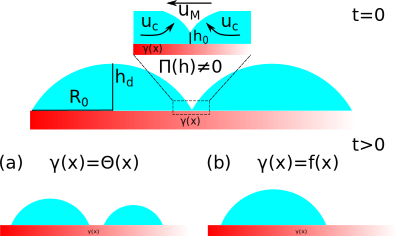
\includegraphics[width=0.48\textwidth]{Figures/setup.png}
    \caption{Schematic setup of the numerical experiment. 
    Two droplets with base radii $R_0$ and maximum height $h_d$ are placed next to each other. 
    They are connected by a liquid bridge with height $h_0$ and subject to a surface tension gradient $\gamma(x)$ (red color gradient).
    The flow has two sizeable contributions, one due to capillarity $u_c$ and one due to Marangoni $u_M$.
    }
    \label{fig:schematics}
\end{figure}
In the presence of a surface tension gradient, Eq.~(\ref{eq:thin_film_simple}) requires another term.
This term accounts for an effective Marangoni flow~\cite{doi:10.1021/la500459v, karpitschka2014sharp, bestehorn20033d, doi:10.1021/la960488a}
\begin{equation}\label{eq:thin_with_marangoni}
    \partial_t h = \partial_x \left(\frac{h^3}{3\mu}\partial_x p + \frac{h^2}{2\mu}\partial_x\gamma\right).
\end{equation}
Naturally, for $\partial_x\gamma = 0$ we retrieve Eq.~(\ref{eq:thin_film_simple}).
These gradients appear due to non-homogenized surfactant concentrations or space resolved heating profiles, e.g. with lasers~\cite{doi:10.1021/la960488a, NIKOLOV2002325, bruning2018delayed, wedershoven2014infrared} or due to different but miscible liquids~\cite{doi:10.1021/la800630w, karpitschka2014sharp, doi:10.1021/la500459v}. 

\subsection{Flows}\label{subsec:flows_theory}
Eq.~(\ref{eq:thin_with_marangoni}) defines the dynamic of the system we are interested in.
Simplifying the equation and setting $\partial\gamma = 0$, we are left with a pure coalescence case.
Following the argumentation of Riegler, Lazar and Eddie et al.~\cite{doi:10.1021/la800630w, PhysRevLett.111.144502} the dynamics in this case is dictated by an strong capillary pressure,
\begin{equation}\label{eq:cap_pressure}
    P_{\text{cap.}} \sim\gamma\kappa \sim \frac{\gamma}{h_0},
\end{equation}
where $\kappa$ is curvature of the liquid vapor interface. 
Having a large curvature at the touching point of the two droplets.
The resulting flow towards the bridge induces a dynamical or ``Bernoulli'' pressure
\begin{equation}\label{eq:P_Bernulli}
    P_{\text{iner.}} \sim \rho v^2 \sim \rho\left(\frac{h_0}{t}\right)^2.
\end{equation}
Balancing Eqs.~(\ref{eq:cap_pressure}-\ref{eq:P_Bernulli}) and solving for $h_0$ yields a growth law 
\begin{equation}\label{eq:coal_powerlaw}
    h_0(t) \propto t^{2/3},
\end{equation}
for contact angles below $\theta < \pi/2$~\cite{PhysRevLett.111.144502, keller2002breaking}.
Recently, a similar growth law for the coalescence of low viscosity liquid lenses has been experimentally observed and theoretically validate, see Hack et al.~\cite{PhysRevLett.124.194502}.

The addition of $\partial\gamma \neq 0$ alters the pressure balance.
Riegler and Lazar associated Eq.~(\ref{eq:P_Bernulli}) with the difference in surface tension~\cite{doi:10.1021/la800630w}
\begin{equation}\label{eq:P_bernulli_riegler}
    P_{B} \sim \rho v^2 \sim \frac{\rho \Delta\gamma^2}{\mu^2}, 
\end{equation}
with the velocity,
\begin{equation}\label{eq:vel_riegler}
    v = \frac{h_0}{\mu}\partial_x\gamma\approx\frac{\Delta\gamma}{4\mu}\theta,
\end{equation}
where $\Delta\gamma = \gamma_1 - \gamma_2$ and $\gamma_i$ are the surface tensions of the two miscible liquids.
Reducing therefore the problem to the absolute value in surface tension contrast.
Karptischka and Riegler later formulated an elegant theoretical explanation for the flow of the non-coalescing twin droplet state~\cite{PhysRevLett.109.066103}.
Assuming a quasistatic thickness ($\partial_t h \approx 0$) and introducing a constant motion proportional to the capillary number 
\begin{equation}\label{eq:sys_cap_vel}
    Ca = \frac{\mu v}{\gamma},
\end{equation} 
that preserves the bridge. 
We proceed similarly, although with two differences. 
Considering the disjoining pressure, but disregard the velocity term $\propto Ca$.
Starting point is Eq.~(\ref{eq:thin_with_marangoni}) in the limit $\partial_t h \approx 0$, 
\begin{equation}\label{eq:pressure_noncoal}
    \frac{h^3}{3\mu}\partial_x p + \frac{h^2}{2\mu}\partial_x\gamma = 0.
\end{equation}
Solving the above equation for the pressure and inserting Eq.~(\ref{eq:pressure}) we have
\begin{equation}\label{eq:thin_film_quasistatic_pressure}
    \partial_x (\gamma\partial_x^2 h + \Pi(h)) = - \frac{3}{2 h}\partial_x\gamma,
\end{equation}
with $\partial_x\Pi(h)$ on the left-hand side.
Splitting the disjoining pressure into a component depending only on surface tension (\textit{and contact angle}) $K(\gamma)$ and one depending on thickness only $H(h)$ we can readily perform the derivative
\begin{align}\label{eq:disj_derivative1}
    \partial_x\Pi(h) &= \partial_x (K(\gamma)H(h)) \nonumber\\
    &= H(h)\partial_\gamma K(\gamma)\partial_x\gamma + K(\gamma)\partial_h H(h)\partial_x h,
\end{align}
inserting Eq.~(\ref{eq:disjoin}) we find $\partial_\gamma K(\gamma) =K(\gamma)/\gamma$ and $\partial_h H(h) = \xi(h)H(h)$.

Rearranging Eq.~(\ref{eq:thin_film_quasistatic_pressure}) and keeping only $\partial_x^3 h$ on the left side yields
\begin{align}\label{eq:h3_pressure}
    \partial_x^3 h = -\frac{1}{\gamma}\left[\left(\frac{3}{2 h} + \partial_x^2 h \right)\partial_x\gamma 
    + \left(\frac{\partial_x\gamma}{\gamma}+\xi(h)\partial_x h\right)\Pi(h)\right].
\end{align}
Clearly if $\Pi(h)\ll 1$ the second term in the square brackets becomes negligible.
However, at the bridge where the film is thin, one expects that the first term dominates.
Taking a look at the orders of $h$, $\Pi(h) \sim h^{-9}-h^{-3}$ we expect a strong contribution to the region around $h_0$.
Knowing $\partial_x^3 h$ we can derive the velocity profile according to Oron et al.~\cite{RevModPhys.69.931}
\begin{equation}\label{eq:Oron_vel}
    u(z) = \frac{z}{\mu}\left[\partial_x\gamma - \left(\frac{z}{2} - h\right)\gamma\partial_x^3 h\right].
\end{equation}
At the vapor fluid interface $z=h$ and upon inserting Eq.~(\ref{eq:h3_pressure}) the velocity becomes
\begin{equation}\label{eq:OronPlus}
     u(h) = \frac{h}{\mu}\left[\left(\frac{1}{4}-\partial_x^2 h\right)\partial_x\gamma - \frac{h}{2}\left( \xi(h)\partial_x h + \frac{\partial_x\gamma}{\gamma}\right)\Pi(h)\right].
\end{equation}
% Given that terms with higher powers in $h$ are small, e.g. $\partial_x^2 h$ and that disjoining pressure is large for small thicknesses.
In fact, Eq.~(\ref{eq:OronPlus}) recovers the result of Karpitschka and Riegler~\cite{PhysRevLett.109.066103}, in the limit $\Pi(h) = \partial_x^2h = 0$ but with a velocity term proportional to $Ca$.
While $\partial_x^2 h$ is $O(h)$ we assume that $\Pi(h)$ is indeed an important contribution at these small scales.

\section{Method}\label{sec:method}
\begin{figure}
    \centering
    \includegraphics[width=0.48\textwidth]{Figures/three_cases.pdf}
    \caption{Final state of the film thickness $h(x)$ after $10^8$ lattice Boltzmann time iterations.
    The three different curves correspond to different surface tensions $\gamma(x)$.
    Simulations with the same initial condition and surface tension difference yield different dynamics based on $\gamma(x)$, see Eqs.~(\ref{eq:gamma_const}, \ref{eq:gamma_tanh}) for details.
    Both axes are normalized using the initial droplet radius.}
    \label{fig:final_state}
\end{figure}
We use computational methods to iteratively solves Eq.~(\ref{eq:thin_with_marangoni}).
On the one hand, to compare with the known growth law Eq.~(\ref{eq:coal_powerlaw}) of millimeter sized drops, we perform simulations using a volume of fluid (VoF) approach.
These results are therefore independent on the choice of modelling parameters in the thin film model and serve as baseline for the growth law. 
On the other hand, to solve the thin film equation, we use a recently developed lattice Boltzmann method (LBM) for thin film flows~\cite{PhysRevE.100.033313, PhysRevE.104.034801}.
This approach is based on the evolution of discrete probability density functions ($f_i$) where
\begin{equation}\label{eq:LBE}
    \begin{split}
        &f_i(x+c^{(i)}\Delta t,t+\Delta t) = \\
        &\left(1 - \frac{\Delta t}{\tau}\right) f_i(x,t) + \frac{\Delta t}{\tau} f_i^{(eq)}(x,t) + w_i \frac{\Delta t}{c_s^2} c^{(i)} F,
    \end{split}
\end{equation}
with $F$ being the total forces acting on the fluid.
We adopt the standard D1Q3 (one-dimensional) scheme with $3$ lattice velocities~\cite{krueger2017}, given by
\begin{equation}\label{eq:speeds}
c^{(i)}  = [0, c, -c], \quad i = 0, 1, 2,
\end{equation}
where the lattice speeds $c=\frac{\Delta x}{\Delta t}$, with weights
\begin{equation}
w_0 = \frac{2}{3},\quad w_{1,2} = \frac{1}{6},
\end{equation}
and the upper bound for information transport, the speed of sound $c_s^2=\frac{c^2}{3}$.
The equilibrium distribution functions $f_i^{(eq)}$ read~\cite{VANTHANG20107373}:
\begin{gather}
    f_{0}^{eq} = h\left(1-\frac{1}{2c^2}gh - \frac{1}{c^2}u^2\right),\nonumber\\
    f_{1}^{eq} = h\left(\frac{1}{4c^2}gh + \frac{1}{2c}u + \frac{1}{2c^2}u^2\right)\label{eq:equilibria},\\
    f_{2}^{eq} = h\left(\frac{1}{4c^2}gh - \frac{1}{2c}u + \frac{1}{2c^2}u^2\right),\nonumber
\end{gather}
where $g$ is the gravitational acceleration that enforces the hydrostatic pressure condition. 
Given the size of the droplet we are interested in, we neglect gravity and set $g=0$ for the remainder of this work.

The film thickness $h$ and the velocity at the free surface $u$ are moments of the distribution functions $f_i$~\cite{Salmon:1999:0022-2402:503, PhysRevE.65.036309, PhysRevE.104.034801}:
\begin{equation}\label{eq:hydrofields}
    h= \sum_{i=0}^2 f_i \qquad hu = \sum_{i=0}^2 c^{(i)} f_i.
\end{equation}
The force $F$ in (\ref{eq:LBE}) accounts for three terms,
\begin{equation}\label{eq:force}
    F = F_{\text{cap}} + F_{\text{fric}} + F_{\gamma}.  
\end{equation}
First being the effect of the film pressure $p$, Eq.~(\ref{eq:pressure}), 
\begin{equation}\label{eq:capillary_force}
    F_{\text{cap}} = -\frac{1}{\rho_0} h \frac{\partial p}{\partial x},
\end{equation}
($\rho_0$ being the fluid density). 
Viscous friction with the substrate is contained in
\begin{equation}\label{eq:fric_force}
    F_{\text{fric}} = -\nu \alpha_{\delta}(h) u,
\end{equation}
where $\nu=\mu/\rho_0$ is the fluid kinematic viscosity (related to the relaxation time $\tau$ by $\nu = c_s^2\left(\tau-\frac{\Delta t}{2}\right)$).
The thickness dependent function $\alpha_{\delta}(h)$ is approximately an inverse mobility $m(h)$,
\begin{equation}\label{eq:fric_alpha}
     \alpha_{\delta}(h) = \frac{6 h}{2h^2 + 6h\delta + 3\delta^2},
\end{equation}
with a slip length $\delta$.
The surface tension gradient requires the addition of another forcing contribution $F_{\gamma}$.
Similarly to ref~\cite{PhysRevE.104.034801} we construct a force term and match it to the last term in Eq.~\ref{eq:thin_with_marangoni}, 
\begin{equation}\label{eq:force_gamma_grad}
    F_{\gamma} = \frac{3}{2}\partial_x\gamma(x),
\end{equation}
where we have assumed that the surface tension only varies along the horizontal dimension.
It can be shown that the system of Eqs. (\ref{eq:LBE}-\ref{eq:force_gamma_grad}) represent a solver for the system
\begin{equation}\label{eq:lubr2eq1surf}
\begin{cases}
\begin{array}{ll}
\partial_t h + \partial_x (h u)  = 0 & \\ 
\partial_t (h u) = -\frac{1}{\rho_0}h\partial_x p -\nu\alpha_{\delta}(h)u + \frac{3}{2}\partial_x\gamma.
\end{array}
\end{cases}
\end{equation}

Performing the limits discussed in ref.~\cite{PhysRevE.100.033313, PhysRevE.104.034801}, this system is an effective solver for Eq~(\ref{eq:thin_with_marangoni}).
There is however a difference to the model used in refs.~\cite{doi:10.1021/la500459v, karpitschka2014sharp}.
The inclusion of the disjoining pressure allows testing the non-coalescence criteria for smaller scales, well below $1mm$ droplet diameter~\cite{karpitschka2014sharp}.

For the surface tension field, $\gamma(x)$ we use three different functions.
First being just a constant surface tension, 
\begin{equation}\label{eq:gamma_const}
    \gamma^{\text{const.}}(x) = \gamma_0,
\end{equation}
with $\gamma_0$ as constant and therefore $\partial_x\gamma(x) = 0$.
Second, to mimic a mixture of different liquids or a locally heated and cooled substrate, we use a Heaviside function
\begin{equation}\label{eq:gamma_step}
    \gamma^{\text{step}}(x) = \begin{cases}
    \gamma_0\quad~~\qquad \text{for $x < L/2$}\\
    \gamma_0 - \Delta\gamma \quad \text{for $x \ge L/2$}\\
    \end{cases},
\end{equation}
with $\Delta\gamma$ being some percentage of $\gamma_0$.
The third function interpolates smoothly between the two values $\gamma_0$ and $\gamma_0 -\Delta\gamma$ using a tangent hyperbolicus
\begin{align}\label{eq:gamma_tanh}
    \gamma^{\text{smooth}}(x) &= \gamma_0\abs{1 - \left(\frac{1}{2} - s(x;l,w)\right)} + \nonumber\\
    &(\gamma_0 - \Delta\gamma)\left\{1 - \abs{1 - \left(\frac{1}{2} - s(x;l,w)\right)}\right\} 
\end{align}
where
\begin{equation}\label{eq:smoothing}
    s(x;l,w) = \frac{1}{2}\tanh\left(\frac{x - l}{w}\right),
\end{equation}
with $l$ being a coordinate where $\gamma^{\text{smooth}}(l) = \gamma_0 -\Delta\gamma/2$ and $w$ a smoothing width. 
For the rest of manuscript, we keep $l=L/2$ fixed and use the notation $s(x;w)$.
The surface tension effectively enters the LBM through Eqs~(\ref{eq:pressure}-\ref{eq:disjoin}) and Eq.~(\ref{eq:force_gamma_grad}).
In Fig.~\ref{fig:final_state} we display the film thicknesses at time step $t = 10^8\Delta t$ using three different surface tensions.
% The spatially resolved value of the surface tension is then given to the pressure, see .

\section{Results}\label{sec:results}
\begin{figure}
    \centering
    \includegraphics[width=0.48\textwidth]{Figures/bridge_evo_all_2.pdf}
    \caption{Time evolution of the liquid bridge $h_0(t)$ normalized with $R_0$. 
    Different symbols mark different surface tension gradients.
    The black dashed line displays $f(x) = \beta t^{2/3}$, with $\beta \approx 0.01$.}
    \label{fig:bridge_growth}
\end{figure}
First, let us introduce the parameters of our LBM simulations and the relevant length and time scales for both VoF and LBM.
All experiments start with the same initial condition, two barely overlapping circular segments (equivalent to spherical caps in three dimensions) as illustrated in Fig.~\ref{fig:schematics}.
The grid size is $L=1024\Delta x$ with periodic boundary conditions except for $\partial_x\gamma(0) = \partial_x\gamma(L) = 0$.
Both droplets have a base radius $R_0 = 171\Delta x$, a maximum thickness $h_d = 30.15$ and form a contact angle $\theta = \pi/9$ with the substrate.
The initial bridge height is measured to be $h_0(0) \approx 0.2$.
The relaxation time is set to unity, which results in a viscosity $\mu = 1/6$. 
We use a slip boundary condition, see Eq.~(\ref{eq:fric_alpha}), with $\delta \approx h_0/2$.
The surface tension $\gamma_0 = 10^{-5}$, while $\Delta\gamma = 2\cdot 10^{-6}$.
In the disjoining pressure, Eq.~(\ref{eq:disjoin}) we set $h_{\ast} = 0.09$ and $(n,m) = (9,3)$.
% All quantities are given in $l.b.u$ so-called lattice Boltzmann units.

We use the radius of the initial droplets $R_0$ to normalize length scales~\cite{PhysRevLett.111.144502, PhysRevLett.95.164503}.
As a characteristic time scale we use the inertio-capillary time 
\begin{equation}\label{eq:inertio-cap-time}
    \tau_{\text{ic.}} = \sqrt{\frac{\rho R_0^3}{\gamma}}.
\end{equation}
Inserting numbers we get $\tau_{\text{ic.}} \approx 7\cdot 10^5 \Delta t$ for $\gamma=\gamma_0$. 

\subsection{Bridge growth}\label{subsec:growth}
The liquid bridge between two similar drops on a solid substrate with contact angle $\theta < \pi/2$ is expected to grow according to Eq.~(\ref{eq:coal_powerlaw}). 
Initially, this growth law has been derived for macroscopic drops for which the disjoining pressure is irrelevant.
Performing VoF simulations of hexadecan using OpenFOAM, with constant contact angle boundary condition, we find good agreement with Eq.~\ref{eq:coal_powerlaw}.
Interestingly, the same growth rate holds true in our LBM simulations with $\Pi(h) \neq 0$ shown by blue bullets in Fig.~\ref{fig:final_state}-\ref{fig:bridge_growth}.
Only for late stages of the coalescence where $h_0 \sim h_d$ we observe a deviation from the black dashed line give by
\begin{equation}\label{eq:fit_powerlaw}
    f(t) = \beta t^{2/3},
\end{equation}
with $\beta = 0.01$.
The powerlaw is however fairly dependent on the slippage parameter $\delta$. 
For a $\delta \ll h_d$ the velocity boundary condition requires a slow flow close to the fluid substrate boundary, see Eq.~(\ref{eq:fric_alpha}). 
Meaning that the flow into the bridge region is suppressed, and therefore $\alpha < 2/3$.
 
Different choices for $\gamma(x)$ act quite severely on the bridge growth.
Using Eq.~(\ref{eq:gamma_step}) instead of Eq.~(\ref{eq:gamma_const}) is shown by orange diamonds in Fig.~\ref{fig:bridge_growth}.
Clearly, the bridge does not grow, and the droplets do not coalesce.
While there is no concentration field in our simulations, the results qualitatively agree with references~\cite{karpitschka2014sharp, doi:10.1021/la500459v, PhysRevLett.109.066103, doi:10.1021/la800630w}. 
Including $\Pi(h) \neq 0$ the bridge even decreases, leaving only a thin precursor layer ($h\sim h_{\ast}$) between the droplets.
Instead of a steady motion of the twin droplet state, the droplet on the lower surface tension side, therefore $\gamma_0 - \Delta\gamma$ moves away from the step. 
Resulting in a new equilibrium where $\partial_x\gamma = 0$.
This is expected because $\partial_x\gamma\neq 0$ induces a force which results in a flow, see Eq.~(\ref{eq:thin_with_marangoni}).

Smearing out the surface tension gradient using Eq.~(\ref{eq:gamma_tanh}) is shown by the remaining symbols in Fig~\ref{fig:bridge_growth}.
Instead of an immediate separation of the droplets and independent of $w$, see Eq.~(\ref{eq:smoothing}) (different colors and symbols), the bridge starts to grow initially.
More surprisingly, the growth rate is in agreement with the powerlaw $\propto t^{2/3}$ of Eq.~(\ref{eq:coal_powerlaw}).
The droplet on the higher surface tension side is sucking fluid from the lower surface tension one.
This has been observed and explained in ref~\cite{PhysRevLett.109.066103} for $\Pi(h) = 0$.
The subtle difference in our setup is, that the twin droplet system is not supported by a constant velocity.
Instead, we solely rely on the balance between $\Pi(h)$ and $\partial_x\gamma(x)$.
Our understanding is that the system has one global energy minimum, which a single droplet on the high surface tension side.
A local energy minimum is however found when the droplets separate.
This can be seen in Fig.~\ref{fig:final_state} orange stars or in Fig.~\ref{fig:bridge_growth} when the symbols start to deviate from the dashed line.
The bridge height ($h_0(t)$) reaches a maximum and decreases rapidly to $h_0(t) \approx h_{\ast}$.
An effect that can not be explained without considering the disjoining pressure Eq.~(\ref{eq:disjoin}) and the resulting flow Eq.~(\ref{eq:OronPlus}).
Interestingly, the separation time scale seems to be linearly dependent on $w$.

\subsection{Separation and asymmetric coalescence}\label{subsec:separation}
\begin{figure}
    \centering
    \includegraphics[width=0.48\textwidth]{Figures/hdiff.pdf}
    \caption{Difference between the maxima of the two droplets.
    In blue, we supply the symmetric coalescence using $\gamma(x) = \gamma_0$.
    The other curves are subject to a surface tension gradient, with different symbols and colors show different $\gamma(x)$.
    %Up to a smearing width of $w < 50$ all curves collapse to singe one at small time scales.
    }
    \label{fig:drop_diff}
\end{figure}
The evolution of the bridge and therefore the flow is highly sensitive to the surface tension $\gamma(x)$, see Figs~\ref{fig:final_state},\ref{fig:bridge_growth}.
Choosing a constant surface tension $\gamma(x) = \gamma_0$, almost all data is in agreement with $\propto t^{2/3}$.
Given Eqs.~(\ref{eq:gamma_step}-\ref{eq:gamma_tanh}) the less smeared the transition in the surface tension is, the sooner the bridges deviate from the powerlaw.
Turning the argument around, the more space the transition between $\gamma_0$ and $\gamma_0-\Delta\gamma$ can occupy, the longer growth agrees with $\propto t^{2/3}$.
Two things are happening, the first is being that the bridge is moving.
The point of minimal thickness between the droplets shifts its location towards smaller surface tension.
While fluid is flowing in the direction of higher surface tension, the bridge is travelling downstream.

This behavior is more pronounced for larger smearing values $w$.
Increasing $w$ yields smaller $\partial_x\gamma$ values at the bridge, as can be computed using Eq.~(\ref{eq:gamma_tanh}). 
Interestingly, for $w\gtrsim R_0$ we no longer see a separation, but an asymmetric coalescence.
Which is a consequence of traveling bridge and the mass transport.
A simpler measure to assess this statement is the difference in droplet height,
\begin{equation}\label{eq:drop_diff_h}
    \Delta h = |h_{d,1} - h_{d,2}|
\end{equation}
where $h_{d,i}$ with $i=1,2$ identifies the left and right droplet, respectively.
These measurements are shown in Fig.~\ref{fig:drop_diff} for a subset of chosen surface tension fields.
For $w < 50$ or $w/R_0 \le 1/3$ we observe a collapse of the data on short time scales.
The same curves, leaving aside the constant surface tension, show a kink in their slope.
This change is due to the separation and the limited transport in the precursor layer.
Best seen by the yellow triangles where at $t \approx 85$ a kink appears, after which the difference is only growing slowly.
For larger smearing, therefore $w > 50$ we find the system in a transition between asymmetric coalescence and late time separation.
% Meaning that $\partial_x h$ does not change sign between the two droplets, due to $h_d \approx h_0$ for one of the droplets. 

\begin{figure}
    \centering
    \includegraphics[width=0.48\textwidth]{Figures/pressures_three_gam_end.pdf}
    \caption{Pressure distribution around the bridge for three different $\gamma(x)$, Eq.~(\ref{eq:pressure}).
    Solid lines with bullets display the capillary contribution $\partial_x^2 h$ while dashed lines with stars show the disjoining component, Eq.~(\ref{eq:disjoin}.
    On the y-axis we normalize the pressures with $p_0$, see Eq.~\ref{eq:pressure_norm}.
    The x-axis shows the center of the domain $l$ and $\approx R_0$ to the left and the right.
    In the inset, we zoom into the region at $P/p_0 \approx 0$. 
    For $\gamma(x) = s(x;100)$ (green curves) the disjoining pressure is vanishing.}
    \label{fig:pressures}
\end{figure}
To have a better understanding of this process, we measure the two pressure components $\partial_x^2 h$ and $\Pi(h)$, as shown in Fig.~\ref{fig:pressures}.
The full (dashed) lines with bullets (stars) show $\gamma(x)\partial_x^2 h$ ($\Pi(h)$). 
Different colors refer to different $\gamma(x)$s, with all data being from the same time step at $t\approx 130\tau$.
To normalize both pressure components, we use 
\begin{equation}\label{eq:pressure_norm}
    p_0 = \frac{\gamma}{R},
\end{equation}
with $\gamma = \gamma_0$ and $R = R_0$.
Knowing that the coalescence is driven by capillarity ($\gamma\partial_x^2 h$) we expect that $\partial_x^2 h > \Pi(h)$ for $\gamma(x) = \gamma_0$.
Interestingly, already for the smearing $w=100$ this inequality holds true, which is shown in the inset of Fig.~\ref{fig:pressures}.
Reducing the smearing and having a sharp surface tension transition, the disjoining pressure becomes the dominating pressure contribution.
% The blue dashed line, for example, the large negative $\Pi(h)$, induces a flow from positive to negative $x$ values.
While the value is large, the thickness of the precursor layer only allows for a limited flow. 
Still, we argue that at small scales ($R_0 \approx 1\mu m$) the disjoining pressure does influence the coalescence behavior quite significantly.
Lastly, the reduction in scale yields one further difference to, e.g. ref.~\cite{karpitschka2014sharp}.
The statement that the coalescence or non-coalescence is only depending on the absolute surface tension difference ($\gamma_0-\Delta\gamma$) does not hold true.
Instead, one $\Delta\gamma$ can either lead to separation, yellow hexagons Fig.~\ref{fig:bridge_growth} and green hexagons Fig.~\ref{fig:drop_diff} or asymmetric coalescence, see cyan pentagons Fig.~\ref{fig:bridge_growth}.
Of course, assuming that it is possible to have highly controllable surface tension field.

\section{Summary and Conclusions}\label{sec:sum_conclu}

To summarize, we have performed numerical experiments of sessile droplet coalescence using a lattice Boltzmann method based on the thin film equation with an effective Marangoni contribution.
The droplets were subject to a spatially resolved surface tension gradient and a disjoining pressure $\Pi(h)$.
Making strong assumptions on the theoretical formulation, i.e. quasi static profile, we have shown that the disjoining pressure contribution effects the flow.
If there is however no surface tension gradient, the disjoining pressure does not alter the known scaling law for the bridge growth $h_0(t) \propto t^{2/3}$.

Using $\gamma(x)$ we observe two different scenarios.
From references experiments at larger scales with different but miscible liquids, we know that the Marangoni flow can prevent coalescence.
This behavior translates to the first scenario, where the bridge even decreases in height and the droplets separate.
Interestingly, the bridge evolution strongly dependent on the concrete choice of $\gamma(x)$.
Using a step function between the two plateau values, the bridge quickly decreases, and the coalescence process is stopped.
Smearing the step using a tangent hyperbolicus we have a transient bridge growth that for small smearing widths still ends in separation.
Although with a finite mass flux from one droplet into the other.

If the smearing width becomes large ($\approx R_0$) the resulting flow promotes an asymmetric coalescence.
Similar to $\gamma(x) = const.$ the finial state is a single droplet.
In contrast to a constant surface tension, the center of mass of this droplet is clearly shifted towards an area of higher surface tension.
% The reason for this is a combination of capillary flow, thus bridge growth and mass transport due to Marangoni. 

Somewhat surprising is the influence of exact choice of $\gamma(x)$.
Our results can not be explained, having the absolute difference in surface tension as parameter only.
% To the best of our knowledge this statement is true, if we reduce the difference in surface tension coalescence is promoted.
Given the same difference in $\gamma(x)$ we find two solutions, separation and asymmetric coalescence.

In future work, we plan to perform simulations at larger scales using the volume of fluid method.
Therefore, having numerical experiments at scales where the disjoining pressure can be neglected.
Using a similarly well resolved surface tension gradient, we assume to confirm the case of asymmetric coalescence at larger scales.

\begin{acknowledgements}

\end{acknowledgements}


%\input{|python your_script.py}

%\appendix
%\section{}\label{app:one}

\bibliography{Ref}

\end{document}